%============================================================
En este Anexo se presentarán todos los cálculos necesarios para el dimensionamiento de los componentes electrónicos de los circuitos de control y sensado.

%============================================================
\section{Diseño total del canal de relé}
\label{sec:diseno_total_canal_rele}

La Figura~\ref{fig:canal_rele_total} muestra el canal de accionamiento del relé, el cual es controlado mediante una señal GPIO del microcontrolador. Para el aislamiento y protección de la etapa de control se emplea el optoacoplador PC817, cuya salida acciona la etapa de potencia a través de un transistor NPN 2N3904. De este modo, el 2N3904 permite conmutar la bobina del relé de manera segura, manteniendo separadas la electrónica de control y la carga asociada al accionamiento.

\begin{figure}[H]
    \centering
    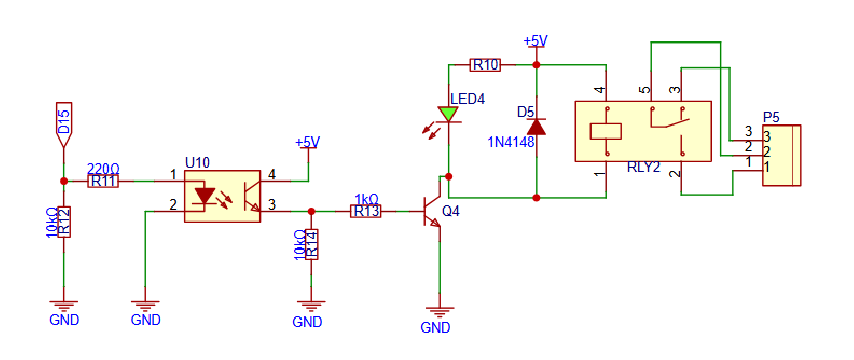
\includegraphics[width=0.88\linewidth]{ANNEX/Fig/AU/CANAL.pdf}
    \caption{Canal total de accionamiento del relé con optoacoplador PC817 y transistor 2N3904.}
    \label{fig:canal_rele_total}
\end{figure}

Cuando la salida del ESP32 se encuentra en nivel lógico bajo, el diodo emisor de luz del optoacoplador no conduce, por lo que el fototransistor permanece en corte y no circula corriente hacia la base del transistor 2N3904. En esta condición, las resistencias de \textit{pull-down} fijan un valor lógico determinado en los nodos de control y de base, manteniendo el transistor en corte. Este comportamiento se ilustra en la Figura~\ref{fig:canal_rele_corte}.

\begin{figure}[H]
    \centering
    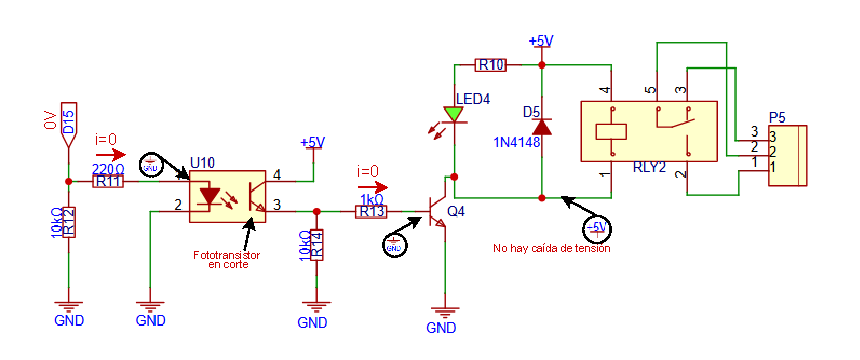
\includegraphics[width=0.88\linewidth]{ANNEX/Fig/AU/corte.pdf}
    \caption{Estado de corte del canal de relé cuando el GPIO del ESP32 se encuentra en nivel lógico bajo.}
    \label{fig:canal_rele_corte}
\end{figure}

A continuación, los cálculos se desarrollan para el estado de saturación de los transistores, iniciando desde el transistor BJT que conmuta el relé, mostrado en la Figura~\ref{fig:canal_rele_etapa_bjt}, y continuando hacia la etapa de aislamiento mediante el optoacoplador, mostrada en la Figura~\ref{fig:canal_rele_etapa_opto}. Para facilitar la referencia, ambas etapas se presentan en la Figura~\ref{fig:canal_rele_etapas}.

\begin{figure}[H]
\centering
\begin{subfigure}[t]{0.48\textwidth}
    \centering
    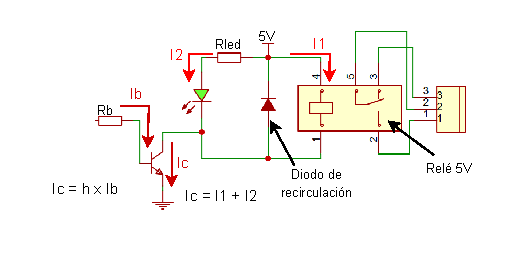
\includegraphics[width=\linewidth]{ANNEX/Fig/AU/Diseno_rele1.pdf}
    \caption{Etapa de conmutación del relé mediante transistor 2N3904.}
    \label{fig:canal_rele_etapa_bjt}
\end{subfigure}
\hfill
\begin{subfigure}[t]{0.48\textwidth}
    \centering
    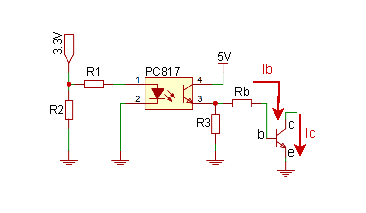
\includegraphics[width=\linewidth]{ANNEX/Fig/AU/Diseno_Rele2.pdf}
    \caption{Etapa de aislamiento mediante optoacoplador PC817.}
    \label{fig:canal_rele_etapa_opto}
\end{subfigure}
\caption{Descomposición del canal de relé en etapa de conmutación y etapa de aislamiento.}
\label{fig:canal_rele_etapas}
\end{figure}
%------------------------------------------------------------
\subsection{Corriente de colector requerida}
\label{subsec:ic_requerida}

Para el dimensionamiento del transistor 2N3904 se parte de la corriente de colector requerida. Por Ley de Corrientes de Kirchhoff en el nodo del colector, la corriente total es la suma de la corriente de la bobina del relé y la corriente del indicador, según la Ecuación~\ref{eq:ic_total}:

\begin{equation}
I_C = I_{\text{2}} + I_{\text{1}}.
\label{eq:ic_total}
\end{equation}

Dado que la bobina del relé demanda aproximadamente \(I_1 = 70~\mathrm{mA}\) y que el indicador LED se diseña con una corriente baja, se asume una corriente de diseño que incluya un margen adicional a la suma de estas corrientes, definida en la Ecuación~\ref{eq:ic_diseno}:

\begin{equation}
I_{C} = 100~\mathrm{mA}.
\label{eq:ic_diseno}
\end{equation}

%------------------------------------------------------------
%------------------------------------------------------------
\subsection{Dimensionamiento de la resistencia del LED \(R_{\text{LED}}\)}
\label{subsec:r_led}

Se considera un LED alimentado desde \(5~\mathrm{V}\) y conmutado a través del transistor 2N3904 operando en saturación. Para el cálculo se requiere la caída colector--emisor en saturación \(V_{CE(sat)}\), la cual se toma de la hoja de datos del 2N3904. En la Figura~\ref{fig:2n3904_vcesat_led} se muestra la característica empleada; para la corriente de operación se adopta \(V_{CE(sat)} = 0.1~\mathrm{V}\) como valor típico y \(V_{CE(sat)} \le 0.2~\mathrm{V}\) como valor máximo. Con el fin de mantener consistencia en la notación, en esta sección la corriente previamente denotada como \(I_2\) se representará como \(I_{\text{LED}}\).

\begin{figure}[H]
    \centering
    % Reemplace el archivo por la figura/recorte del datasheet del 2N3904
    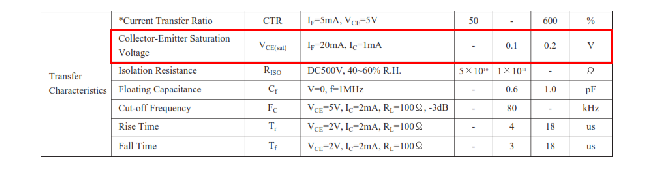
\includegraphics[width=0.78\linewidth]{ANNEX/Fig/AU/Vec_SAT.pdf}
    \caption{Caída colector--emisor del 2N3904 en saturación, \(V_{CE(sat)}\), en función de la corriente de colector.}
    \label{fig:2n3904_vcesat_led}
\end{figure}

Aplicando la Ley de Voltajes de Kirchhoff en la rama del LED se obtiene:

\begin{align}
5~\mathrm{V}-I_{\text{LED}}R_{\text{LED}}-V_{F,\text{LED}}-V_{CE(sat)}=0.
\label{eq:kvl_led}
\end{align}

Despejando \(R_{\text{LED}}\):

\begin{align}
R_{\text{LED}}=\frac{5~\mathrm{V}-V_{F,\text{LED}}-V_{CE(sat)}}{I_{\text{LED}}}.
\label{eq:rled}
\end{align}

Para asegurar visibilidad sin incrementar significativamente el consumo, se adopta una corriente de diseño
\(I_{\text{LED}}\in[2,\,5]~\mathrm{mA}\) y, para un LED típico, \(V_{F,\text{LED}}\in[1.8,\,2.2]~\mathrm{V}\).
De acuerdo con \eqref{eq:rled}, el rango de resistencias se obtiene evaluando los casos extremos:

\begin{align}
R_{\text{LED,min}}
&= \frac{5~\mathrm{V}-1.8~\mathrm{V}-0.1~\mathrm{V}}{5~\mathrm{mA}}
= 620~\Omega,
\label{eq:rled_min}
\\
R_{\text{LED,max}}
&= \frac{5~\mathrm{V}-2.2~\mathrm{V}-0.2~\mathrm{V}}{2~\mathrm{mA}}
= 1300~\Omega.
\label{eq:rled_max}
\end{align}

Con base en el rango de \eqref{eq:rled_min}--\eqref{eq:rled_max}, por serie comercial y compromiso entre visibilidad y consumo se selecciona:

\begin{align}
R_{\text{LED}}=1~\mathrm{k}\Omega.
\label{eq:rled_sel}
\end{align}

%------------------------------------------------------------
\subsection{Corriente de base requerida para saturación del 2N3904}
\label{subsec:ib_requerida}

Para garantizar conmutación, se fuerza una ganancia de corriente conservadora \(h_{fe}\), menor a la ganancia típica observada en hoja de datos a la corriente de operación. Para ello, se emplea la Figura~\ref{fig:2n3904_hfe} como referencia.

\begin{figure}[H]
    \centering
    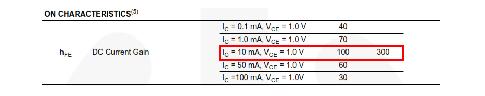
\includegraphics[width=0.90\linewidth]{ANNEX/Fig/AU/current_gain.pdf}
    \caption{Ganancia de corriente en continua del 2N3904, \(h_{FE}\), en función de \(I_C\).}
    \label{fig:2n3904_hfe}
\end{figure}

En este diseño se adopta \(h_{fe} = 30\). Por tanto, la corriente mínima de base para \(I_{C,\text{des}}\) definido en la Ecuación~\ref{eq:ic_diseno} resulta:

\begin{equation}
I_B \ge \frac{I_{C,\text{des}}}{h_{fe}}.
\label{eq:ib_min}
\end{equation}

Sustituyendo \(I_{C,\text{des}}=100~\mathrm{mA}\) en la Ecuación~\ref{eq:ib_min}:

\begin{equation}
I_B = 3.33~\mathrm{mA}.
\label{eq:ib_rango}
\end{equation}

%------------------------------------------------------------
\subsection{Dimensionamiento de la resistencia de base \(R_B\)}
\label{subsec:rb}

La base del 2N3904 se polariza desde el lado aislado a 5~V a través del fototransistor del PC817. Para el cálculo se requieren dos parámetros de hoja de datos:

\begin{itemize}
    \item La caída colector-emisor del fototransistor del PC817 en saturación, \(V_{CE(sat),\text{PC817}}\), tomada de la Figura~\ref{fig:pc817_vcesat}.
    \item La caída base-emisor del 2N3904 en saturación, \(V_{BE(sat)}\), tomada de la Figura~\ref{fig:2n3904_vcesat}.
\end{itemize}
\vspace{-1.25em}
\begin{figure}[H]
    \centering
    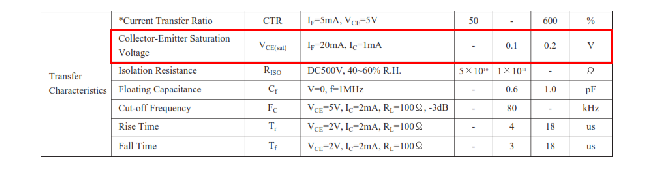
\includegraphics[width=0.98\linewidth]{ANNEX/Fig/AU/Vec_SAT.pdf}
    \caption{Tensión colector-emisor del fototransistor del PC817, \(V_{CE(sat),\text{PC817}}\), en función de la corriente.}
    \label{fig:pc817_vcesat}
\end{figure}
\vspace{-1.25em}
\begin{figure}[H]
    \centering
    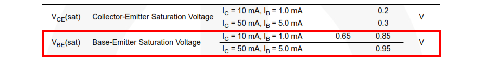
\includegraphics[width=0.98\linewidth]{ANNEX/Fig/AU/Vbe_SAT.pdf}
    \caption{Tensión base-emisor del 2N3904 en saturación, \(V_{BE(sat)}\), en función de \(I_C\).}
    \label{fig:2n3904_vcesat}
\end{figure}

Aplicando la Ley de Voltajes de Kirchhoff en el lazo de excitación de base (referido a 5~V) se obtiene

\begin{equation}
5~\mathrm{V}-V_{CE(sat),\text{PC817}} - I_B R_B - V_{BE(sat)} = 0.
\label{eq:kvl_rb}
\end{equation}

Despejando \(R_B\) de la Ecuación~\ref{eq:kvl_rb}:

\begin{equation}
R_B=\frac{5~\mathrm{V}-V_{CE(sat),\text{PC817}}-V_{BE(sat)}}{I_B}.
\label{eq:rb}
\end{equation}

Adoptando rangos típicos de diseño \(V_{CE(sat),\text{PC817}}\in[0.1,\,0.2]~\mathrm{V}\) y \(V_{BE(sat)}\in[0.85,\,0.95]~\mathrm{V}\), junto con el rango de \(I_B\) de la Ecuación~\ref{eq:ib_rango}, al sustituir en la Ecuación~\ref{eq:rb} se obtiene:

\begin{align}
R_{B,\min} &= \frac{5~\mathrm{V}-0.2~\mathrm{V}-0.95~\mathrm{V}}{3.3~\mathrm{mA}} = 1166.67~\Omega, \\
R_{B,\max} &= \frac{5~\mathrm{V}-0.1~\mathrm{V}-0.85~\mathrm{V}}{3.33~\mathrm{mA}} = 1227.27~\Omega.
\label{eq:rb_rango}
\end{align}

Con base en el rango de la Ecuación~\ref{eq:rb_rango}, por serie comercial y margen de saturación se selecciona:

\begin{equation}
R_B=1.2~\mathrm{k}\Omega.
\label{eq:rb_sel}
\end{equation}

%------------------------------------------------------------
\subsection{Resistencias de \textit{pull-down}}
\label{subsec:pull_down}

Se incorporan resistencias de \textit{pull-down} para asegurar un valor lógico determinado en reposo y evitar nodos flotantes. En particular, una resistencia fija el estado del nodo de entrada del optoacoplador cuando la salida del microcontrolador se encuentra en alta impedancia (arranque o reinicio), y otra resistencia fija el estado del nodo de base del 2N3904 cuando el PC817 no conduce, contribuyendo además a descargar la base.

Seleccionando \(R_2=R_3=10~\mathrm{k}\Omega\), el consumo adicional en estado alto se mantiene bajo:

\begin{equation}
I_{R2}=\frac{3.3~\mathrm{V}}{10~\mathrm{k}\Omega}=0.33~\mathrm{mA},
\qquad
I_{R3}=\frac{5~\mathrm{V}}{10~\mathrm{k}\Omega}=0.5~\mathrm{mA}.
\label{eq:pull_down_corr}
\end{equation}

%------------------------------------------------------------
\subsection{Dimensionamiento de la resistencia \(R_1\) del PC817}
\label{subsec:r1}

La resistencia \(R_1\) limita la corriente del diodo emisor de luz del PC817. Para el cálculo se requiere la tensión directa \(V_{F,\text{PC817}}\), tomada de la Figura~\ref{fig:pc817_vf}.

\begin{figure}[H]
    \centering
    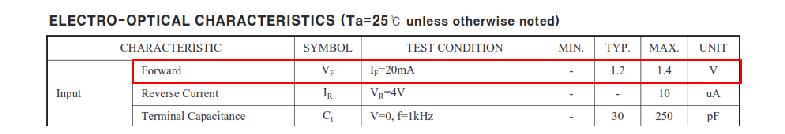
\includegraphics[width=0.98\linewidth]{ANNEX/Fig/AU/V_forward.pdf}
    \caption{Tensión directa del diodo emisor de luz del PC817, \(V_{F,\text{PC817}}\), en función de \(I_F\).}
    \label{fig:pc817_vf}
\end{figure}

Aplicando la Ley de Voltajes de Kirchhoff en el lazo de entrada se obtiene la Ecuación~\ref{eq:kvl_r1}:

\begin{equation}
3.3~\mathrm{V} - I_F R_1 - V_{F,\text{PC817}} = 0.
\label{eq:kvl_r1}
\end{equation}

Despejando \(R_1\) de la Ecuación~\ref{eq:kvl_r1}:

\begin{equation}
R_1=\frac{3.3~\mathrm{V}-V_{F,\text{PC817}}}{I_F}.
\label{eq:r1}
\end{equation}

A partir de la Figura~\ref{fig:pc817_vf} se considera \(V_{F,\text{PC817}}\in[1.2,\,1.4]~\mathrm{V}\). Para una activación robusta del canal se adopta \(I_F\in[8,10]~\mathrm{mA}\). Sustituyendo estos rangos en la Ecuación~\ref{eq:r1}, se obtiene:

\begin{align}
R_{1,\min} &= \frac{3.3~\mathrm{V}-1.4~\mathrm{V}}{10~\mathrm{mA}} = 190~\Omega, \\
R_{1,\max} &= \frac{3.3~\mathrm{V}-1.2~\mathrm{V}}{8~\mathrm{mA}} = 262.5~\Omega.
\label{eq:r1_rango}
\end{align}

Con base en el rango de la Ecuación~\ref{eq:r1_rango}, por serie comercial y margen se selecciona:

\begin{equation}
R_1=220~\Omega.
\label{eq:r1_sel}
\end{equation}
%============================================================


%============================================================
\section{Diseño de filtros y circuitos para el sensado}
\label{sec:diseno_filtros_sensado}

El sistema realiza adquisiciones con un periodo entre muestras de \(500~\mu\mathrm{s}\), lo cual corresponde a una frecuencia de muestreo definida en la Ecuación~\ref{eq:fs_500us}:

\begin{equation}
f_s=\frac{1}{T_s}=\frac{1}{500~\mu\mathrm{s}}=2000~\mathrm{Hz}.
\label{eq:fs_500us}
\end{equation}

Este valor se emplea como referencia para el dimensionamiento de los filtros analógicos, con el objetivo de atenuar componentes de alta frecuencia previas a la digitalización.

%------------------------------------------------------------
\subsection{Divisor resistivo para medición de tensión por ADC}
\label{subsec:divisor_adc}

Se emplea un divisor resistivo para reducir una tensión máxima de 12~V a un nivel compatible con el convertidor analógico digital. La relación del divisor se describe en la Ecuación~\ref{eq:divisor_adc} y se impone la condición de no saturación indicada en la Ecuación~\ref{eq:divisor_adc_cond}.

\begin{equation}
V_{\mathrm{ADC}} = V_{\max}\,\frac{R_{\mathrm{ADC}}}{R_{\mathrm{ADC}} + R_{\mathrm{div}}}.
\label{eq:divisor_adc}
\end{equation}

\begin{equation}
V_{\mathrm{ADC}} < 3.3~\mathrm{V}.
\label{eq:divisor_adc_cond}
\end{equation}

Para el diseño se asume inicialmente \(R_{\mathrm{ADC}}=1~\mathrm{k}\Omega\). Despejando \(R_{\mathrm{div}}\) a partir de la Ecuación~\ref{eq:divisor_adc} y la condición de la Ecuación~\ref{eq:divisor_adc_cond}, se obtiene:

\begin{equation}
R_{\mathrm{div}} > R_{\mathrm{ADC}}\left(\frac{V_{\max}}{V_{\mathrm{ADC,max}}}-1\right).
\label{eq:rdiv_cond}
\end{equation}

Sustituyendo \(V_{\max}=12~\mathrm{V}\), \(V_{\mathrm{ADC,max}}=3.3~\mathrm{V}\) y \(R_{\mathrm{ADC}}=1~\mathrm{k}\Omega\) en la Ecuación~\ref{eq:rdiv_cond}:

\begin{equation}
R_{\mathrm{div}} > \left(\frac{12}{3.3}-1\right) = 2.64~\mathrm{k}\Omega.
\label{eq:rdiv_num}
\end{equation}

Por motivos de seguridad se seleccionan valores mayores, con el fin de reducir el riesgo de aproximarse al límite de 3.3~V. En esta implementación se utilizan \(R_{\mathrm{ADC}}=1~\mathrm{k}\Omega\) y \(R_{\mathrm{div}}=3~\mathrm{k}\Omega\). Sustituyendo en la Ecuación~\ref{eq:divisor_adc}:

\begin{equation}
V_{\mathrm{ADC}} = 12~\mathrm{V}\,\frac{1~\mathrm{k}\Omega}{1~\mathrm{k}\Omega+3~\mathrm{k}\Omega}
= 3~\mathrm{V}.
\label{eq:vadc_num}
\end{equation}

Para definir la potencia requerida en las resistencias se considera el caso de voltaje máximo. La corriente por el divisor está dada por la Ecuación~\ref{eq:div_corr}:

\begin{equation}
I = \frac{V_{\max}}{R_{\mathrm{ADC}}+R_{\mathrm{div}}}.
\label{eq:div_corr}
\end{equation}

Sustituyendo \(V_{\max}=12~\mathrm{V}\), \(R_{\mathrm{ADC}}=1~\mathrm{k}\Omega\) y \(R_{\mathrm{div}}=3~\mathrm{k}\Omega\) en la Ecuación~\ref{eq:div_corr}:

\begin{equation}
I = \frac{12~\mathrm{V}}{4~\mathrm{k}\Omega}=3~\mathrm{mA}.
\label{eq:div_corr_num}
\end{equation}

La potencia disipada en cada resistencia se calcula como \(P=I^2R\). Por tanto, usando el valor de la corriente de la Ecuación~\ref{eq:div_corr_num}:

\begin{align}
P_{R_{\mathrm{ADC}}} &= I^2R_{\mathrm{ADC}} = (3~\mathrm{mA})^2\,1~\mathrm{k}\Omega
= 0.009~\mathrm{W}, \\
P_{R_{\mathrm{div}}} &= I^2R_{\mathrm{div}} = (3~\mathrm{mA})^2\,3~\mathrm{k}\Omega
= 0.027~\mathrm{W}.
\label{eq:pot_div}
\end{align}

En ambos casos la potencia disipada de la Ecuación~\ref{eq:pot_div} es menor que 0.25~W, por lo que resistencias de 0.25~W son suficientes para esta etapa de medición.

%------------------------------------------------------------
\subsection{Acondicionamiento de la señal PWM hacia la entrada PWM del VNH7070BAS}
\label{subsec:pwm_acond}

Para la etapa de control se emplea una señal \ac{PWM} de \(10~\mathrm{kHz}\) hacia la entrada PWM del driver VNH7070BAS. Con el fin de reducir ruido y atenuar componentes de muy alta frecuencia, se incorpora un filtro pasabajos de primer orden tipo RC. Este acondicionamiento no busca suavizar la señal \ac{PWM}, sino limitar el contenido espectral por encima de la banda de interés, manteniendo la integridad del ciclo de trabajo.

La frecuencia de corte del arreglo RC se calcula con la Ecuación~\ref{eq:fc_rc_pwm}:

\begin{align}
f_c&=\frac{1}{2\pi RC}.
\label{eq:fc_rc_pwm}
\end{align}

Para garantizar que la componente fundamental de la señal \ac{PWM} de \(10~\mathrm{kHz}\) se transmita correctamente y, a su vez, atenuar componentes por encima de dicha banda, se selecciona un filtro con \(f_c \geq 15~\mathrm{kHz}\). De la Ecuación~\ref{eq:fc_rc_pwm} se obtiene el producto \(RC\) requerido:

\begin{align}
RC&=\frac{1}{2\pi f_c}
= \frac{1}{2\pi(15\times 10^3)}
= 10.6~\mu\mathrm{s}.
\label{eq:rc_pwm_obj}
\end{align}

Con base en \ref{eq:rc_pwm_obj}, se selecciona una combinación de valores comerciales que cumple \(f_c>15~\mathrm{kHz}\) y mantiene una constante de tiempo pequeña respecto al periodo de la \ac{PWM} (\(T=100~\mu\mathrm{s}\)), minimizando la distorsión del ciclo de trabajo. La selección propuesta se resume en la Ecuación~\ref{eq:rc_pwm_sel}:

\begin{align}
R&=1~\mathrm{k}\Omega, \qquad C=10~\mathrm{nF}
\Rightarrow
f_c=\frac{1}{2\pi(1~\mathrm{k}\Omega)(10~\mathrm{nF})}= 15.9~\mathrm{kHz}.
\label{eq:rc_pwm_sel}
\end{align}

%------------------------------------------------------------
\subsection{Sensado de corriente del VNH7070BAS y filtro previo al ADC}
\label{subsec:cs_vnh7070}

Como se mencionó en el Capítulo~\ref{ch:CH04}, el driver VNH7070BAS permite el sensado de corriente mediante una salida de corriente proporcional a la corriente suministrada al motor. Para ello, siguiendo las recomendaciones de diseño mostradas en la Figura~\ref{fig:diseño_CS}, se implementa una resistencia \(R_{\mathrm{sense}}\) para convertir dicha señal en un voltaje que pueda ser leído por el microcontrolador. Para el diseño de estos circuitos, se utilizará el factor de escalamiento típico de corriente \(K\) de la hoja de datos del \textit{driver} que se muestra en la Figura~\ref{fig:tabla_k}.

Considerando el factor típico \(K\) y la corriente máxima esperada del motor \(I_{\max}\), la corriente de sensado se aproxima como se indica en la Ecuación~\ref{eq:Ics}:

\begin{align}
I_{\mathrm{CS}}&=\frac{I_{\max}}{K}.
\label{eq:Ics}
\end{align}

La conversión a voltaje mediante la resistencia \(R_{\mathrm{sense}}\) se expresa según la Ecuación~\ref{eq:Vcs}:

\begin{align}
V_{\mathrm{CS}}&=I_{\mathrm{CS}}\,R_{\mathrm{sense}}.
\label{eq:Vcs}
\end{align}

Para evitar la saturación de la entrada analógica del microcontrolador se impone la condición de la Ecuación~\ref{eq:cond_sat}:

\begin{align}
V_{\mathrm{CS,max}}&\leq V_{\mathrm{ADC,max}}.
\label{eq:cond_sat}
\end{align}

De las Ecuaciones~\ref{eq:Ics} a \ref{eq:cond_sat} se obtiene el criterio de diseño para \(R_{\mathrm{sense}}\) indicado en la Ecuación~\ref{eq:Rsense_max}:

\begin{align}
R_{\mathrm{sense}}
&\leq \frac{V_{\mathrm{ADC,max}}}{I_{\mathrm{CS,max}}}
= \frac{V_{\mathrm{ADC,max}}\,K}{I_{\max}}.
\label{eq:Rsense_max}
\end{align}

Con \(I_{\max}=8~\mathrm{A}\), \(K=1540\) y \(V_{\mathrm{ADC,max}}=3.3~\mathrm{V}\), sustituyendo en la Ecuación~\ref{eq:Ics} se calcula:

\begin{align}
I_{\mathrm{CS,max}}&=\frac{8~\mathrm{A}}{1540}=5.19~\mathrm{mA}.
\label{eq:Ics_num}
\end{align}

Luego, sustituyendo la Ecuación~\ref{eq:Ics_num} en la Ecuación~\ref{eq:Rsense_max}, resulta:

\begin{align}
R_{\mathrm{sense}}
&\leq \frac{3.3~\mathrm{V}}{5.19~\mathrm{mA}}
= 635~\Omega.
\label{eq:Rsense_num}
\end{align}

En esta implementación se selecciona \(R_{\mathrm{sense}}=500~\Omega\) para incorporar márgenes ante variaciones del factor \(K\) y picos de corriente.

Adicionalmente, se incorpora un filtro pasabajos RC previo al ADC con el fin de reducir picos de alta frecuencia en la señal de sensado. La frecuencia de corte del filtro se determina mediante la Ecuación~\ref{eq:fc_rc_adc}:

\begin{align}
f_c&=\frac{1}{2\pi R_{\mathrm{f}}C_{\mathrm{f}}}.
\label{eq:fc_rc_adc}
\end{align}

Para mantener un ancho de banda suficiente para la dinámica de corriente y, a la vez, atenuar componentes por encima de \(15~\mathrm{kHz}\), se selecciona \(f_c = 15~\mathrm{kHz}\). Por tanto,

\begin{align}
R_{\mathrm{f}}C_{\mathrm{f}}
&=\frac{1}{2\pi f_c}
= \frac{1}{2\pi(15\times 10^3)}
= 10.6~\mu\mathrm{s}.
\label{eq:rc_adc_obj}
\end{align}

Con base en \ref{eq:rc_adc_obj}, se selecciona una combinación de valores comerciales para el filtro previo al ADC, la cual se resume en la Ecuación~\ref{eq:rc_adc_sel}:

\begin{align}
R_{\mathrm{f}}&=1~\mathrm{k}\Omega, \qquad C_{\mathrm{f}}=10~\mathrm{nF}
\Rightarrow
f_c=\frac{1}{2\pi(1~\mathrm{k}\Omega)(10~\mathrm{nF})}= 15.9~\mathrm{kHz}.
\label{eq:rc_adc_sel}
\end{align}

\begin{figure}[H]
\centering
\begin{subfigure}[t]{0.48\textwidth}
\centering
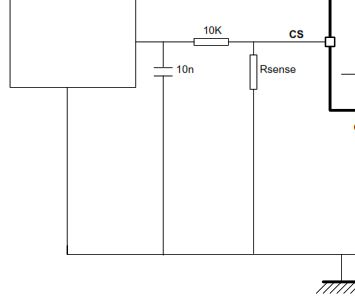
\includegraphics[width=\linewidth]{CHPTRS/CH07_IMPLEMENTACION/Fig/DISEÑO_CS.JPG}
\caption{Recomendación de implementación del sensado CS.}
\label{fig:diseño_CS}
\end{subfigure}
\hfill
\begin{subfigure}[t]{0.48\textwidth}
\centering
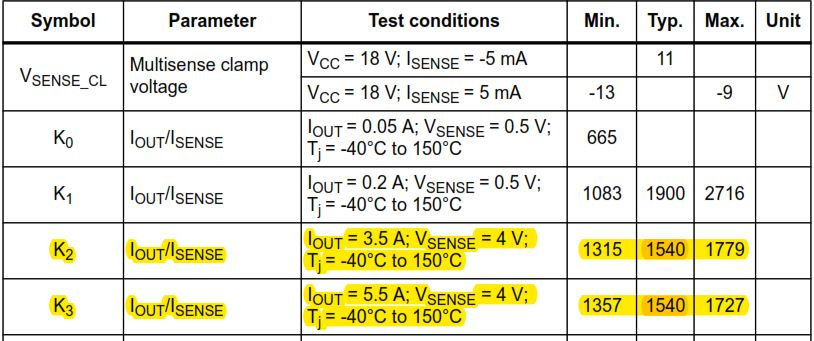
\includegraphics[width=\linewidth]{CHPTRS/CH07_IMPLEMENTACION/Fig/K0.JPG}
\caption{Tabla del factor de escalamiento típico de corriente.}
\label{fig:tabla_k}
\end{subfigure}
\caption{Recomendaciones de la hoja de datos para el sensado de corriente con el VNH7070BAS.}
\label{fig:cs_datasheet}
\end{figure}
%============================================================
